%Copyright 2014 Jean-Philippe Eisenbarth
%This program is free software: you can 
%redistribute it and/or modify it under the terms of the GNU General Public 
%License as published by the Free Software Foundation, either version 3 of the 
%License, or (at your option) any later version.
%This program is distributed in the hope that it will be useful,but WITHOUT ANY 
%WARRANTY; without even the implied warranty of MERCHANTABILITY or FITNESS FOR A 
%PARTICULAR PURPOSE. See the GNU General Public License for more details.
%You should have received a copy of the GNU General Public License along with 
%this program.  If not, see <http://www.gnu.org/licenses/>.

%Based on the code of Yiannis Lazarides
%http://tex.stackexchange.com/questions/42602/software-requirements-specification-with-latex
%http://tex.stackexchange.com/users/963/yiannis-lazarides
%Also based on the template of Karl E. Wiegers
%http://www.se.rit.edu/~emad/teaching/slides/srs_template_sep14.pdf
%http://karlwiegers.com
\documentclass{scrreprt}
\usepackage{listings}
\usepackage{underscore}
\usepackage[bookmarks=true]{hyperref}
\usepackage[utf8]{inputenc}
\usepackage[english]{babel}
\usepackage{array}
\usepackage{graphicx}
\usepackage{fancybox,fancyhdr}
\usepackage{setspace}
\onehalfspacing
\fancyhead[R]{\today}
\fancyhead[L]{SRS V 1.0}
\renewcommand{\chapterheadstartvskip}{\vspace{0cm}}
\usepackage[left=2cm,right=2cm,
    top=2cm,bottom=3cm,bindingoffset=0cm]{geometry}
\hypersetup{
    bookmarks=false,    % show bookmarks bar?
    pdftitle={Software Requirement Specification},    % title
    pdfauthor={User},                     % author
    pdfsubject={TeX and LaTeX},                        % subject of the document
    pdfkeywords={TeX, LaTeX, graphics, images}, % list of keywords
    colorlinks=true,       % false: boxed links; true: colored links
    linkcolor=blue,       % color of internal links
    citecolor=black,       % color of links to bibliography
    filecolor=black,        % color of file links
    urlcolor=purple,        % color of external links
    linktoc=page            % only page is linked
}%
\def\myversion{1.0 }
\date{}
%\title
\usepackage{hyperref}
\fancypagestyle{plain}{
\fancyhead[R]{\today}
\fancyhead[L]{SRS V 1.0}
\fancyheadoffset{0mm}
}
\setlength{\parindent}{0cm}
\usepackage{parskip}
\begin{document}
\begin{flushright}
   \rule{16cm}{5pt}\vskip1cm
    \begin{bfseries}
        \thispagestyle{empty} %do not number the title page
        \begin{center}
        \Huge{SOFTWARE REQUIREMENTS\\ SPECIFICATION}\\
        for\\
        \vspace{1.9cm}
        Android application\\ "Fluber"\\
        \vspace{1.9cm}
        \LARGE{Version \myversion approved}\\
        \vspace{1.9cm}
        \end{center}
        Prepared by \\
        
        Babich Kirill\\
        Beryukhov Andrey\\
        Klochkiv Lev\\
        Repina Anastasia\\

        \vspace{1.9cm}
        \today\\
    \end{bfseries}
\end{flushright}


\tableofcontents
\setcounter{page}{1}

\pagestyle{fancy} 
\chapter{Introduction}
\section{Purpose}
The purpose of this document is to present a detailed description of the “Fluber” application for Android. It will explain the purpose and features of the system, the interfaces of the system, what the system will do, the constraints under which it must operate and how the system will react to external stimuli. This document is intended for the developers of the application and end-users.

\section{Scope of the product}
People who buy flowers do not have an opportunity to compare the prices for the bouquets in the nearest shops of the district when they are already in the shop, as this data is not agregated and availiable. To let users choose the best option and buy the best bouquets for the cheapest price correct their timetable we give them an opportunity to make an order inside the application. Flower suppliers will be able to add their shops to the application base, so both: buyer and seller will be in positive territory. It should increase flower shops revenue and help people to make the choise.

The application contains a relational database containing a list of Shops, Users, Flowers, Orders.

\section{ Definitions, acronyms and abbreviations}
\begin{tabular}{| m{4cm} | m{10cm} |}
	\hline
	\textbf{Term} & \textbf{Definition} \\ \hline
	API & A set of subroutine definitions, protocols, and tools for building software and applications.  \\ \hline
	Database &  Collection of all the information monitored by this system.\\ \hline
	Field  & A cell within a form. \\ \hline
	Software Requirements Specification & 
	A document that completely describes all of the functions of a proposed system and the constraints under which it must operate. For example, this document. \\ \hline
	Buyer & A person, who buy flowers and make an order in the application. \\ \hline
	Seller & A person, who sell flowers and get orders in the application. \\ \hline
	User & See Buyer and Seller\\
	\hline
\end{tabular}

\section{References}
IEEE. IEEE Std 830-1998 IEEE Recommended Practice for Software Requirements Specifications. IEEE Computer Society, 1998.

\section{Overview of the document}
The next chapter, the Overall Description section, of this document gives an overview of the functionality of the product. It describes the informal requirements and is used to establish a context for the technical requirements specification in the next chapter.
The third chapter, Functional Requirements section, of this document is written primarily for the developers and describes in technical terms the details of the functionality of the product.
The fourth chapter, Non-functional Requirements section, of this document is about specify criteria that can be used to judge the operation of a system, rather than specific behaviors.
The last chapter is Other Requirements, which contains  requirements not covered elsewhere in the SRS.
All sections of the document describe the same software product in its entirety, but are intended for different audiences and thus use different language.

\chapter{Overall Description}

This section will give an overview of the whole system. The system will be explained in its context to show how the system interacts with other systems and introduce the basic functionality of it. It will also describe what type of stakeholders that will use the system and what functionality is available for each type. At last, the constraints and assumptions for the system will be presented.

\section{Product Perspective}
This system is an Android application, which will be used to make and fullfill orders for flowers, view information about them. The mobile application will need an access to the Internet in order to use Firebase API to work with database and Google Maps API, which allows to find out all shops locations. Diagram below shows, how different modules interacts, see Figure 1.

\begin{center}
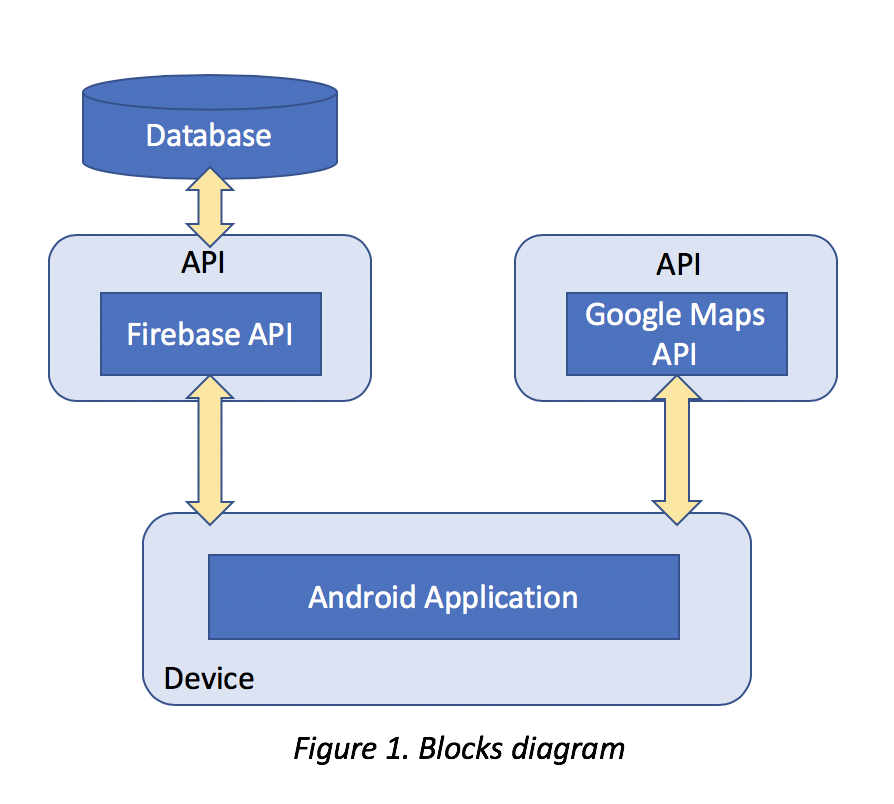
\includegraphics[scale=0.7]{blocks}
\end{center}
Since this is a data-centric product, it will need somewhere to store the data. For that, a database will be used. A mobile application will communicate with the database via Firebase API. In database it will send, get and modify data.

The mobile application has no restrictions about the resource allocation.

\section{Product Functions}
\begin{itemize}
\item Flowers sale (for gardener - sellers)
\item Flowers purchase (for clients - buyers)
\item Filtration the results (to find the best variant)
\item Geotracking the sellers around and showing on Google map
\item Tracking the orders using notifications
\item Ability to pay for order inside application
\end{itemize}

All changes will be saved and stored in database.  

\section{User Classes and Characteristics}
There are two types of users that interact with the system: buyers and sellers. They have different interaction plans with the application. Users main goal is to post an order and get the flowers, whereas sellers after adding their shop to the shops database can fullfill the customer orders. 

\section{Constraints}
The mobile application is constrained by the Internet, because of filling database. 

\section{User Documentation}
No user documentation is planned.

\section{Assumptions and Dependencies}

One assumption about the product is that it will always be used on mobile phones that have enough performance. If the phone does not have enough hardware resources available for the application, for example, the users might have allocated them with other applications; there may be scenarios where the application does not work as intended or even at all.

\chapter{Specific requirements}
\section{External Interface Requirements}

\subsection{User Interfaces}
A first-time user of the mobile application should see the empty timetable page when he/she opens the application. If the user has not registered, he/she should open the menu, see Figure 1, and be able to do that on the search page, see Figures 2 and 3.
If the user is not a first-time user, he/she should be able to see the timetable page directly with his/her own timetable when the
application is opened, see Figure 4.   Also, it is possible to find all the campuses and all the buildings on the map page, see Figure 6. The information about the application can be found on the info page, see Figure 7.

\begin{figure}[h]
\begin{minipage}[h]{0.32\linewidth}
\center{\includegraphics[width=0.8\linewidth]{menu.png} \\ Figure1. Menu in navigation drawer}
\end{minipage}
\hfill
\begin{minipage}[h]{0.32\linewidth}
\center{\includegraphics[width=0.8\linewidth]{searchstudent.png} \\Figure 2. Search page for student}
\end{minipage}
\begin{minipage}[h]{0.32\linewidth}
\center{\includegraphics[width=0.8\linewidth]{searchprofessor.png} \\Figure 3. Search page for professor}
\end{minipage}
\end{figure}
\begin{figure}[h]
\begin{minipage}[h]{0.32\linewidth}
\center{\includegraphics[width=0.8\linewidth]{timetable.png} \\ Figure 4. Timetable page}
\end{minipage}
\hfill
\begin{minipage}[h]{0.32\linewidth}
\center{\includegraphics[width=0.8\linewidth]{settings.png} \\Figure 5. Settings page}
\end{minipage}
\begin{minipage}[h]{0.32\linewidth}
\center{\includegraphics[width=0.8\linewidth]{map.png} \\Figure 6. Map page}
\end{minipage}
\end{figure}
\begin{figure}[h]
\center
{\includegraphics[width=40mm]{info.png} \\Figure 7. Info page}
\end{figure}

\newpage
\subsection{Hardware Interfaces}
Since the mobile application doesn't have any designated hardware, it does not have
any direct hardware interfaces. The physical GPS is managed by the GPS application in the mobile phone
and the hardware connection to the database server is managed by the underlying operating system on the
mobile phone.

\subsection{Software Interfaces}
The mobile application communicates with the GPS application in order to get geographical information
about where the user is located and the visual representation of it, with RUZ system to get timetables
and with the local database in order to save and edit timetables, see Figure 1. The communication between
the database and the mobile application consists of operation concerning both reading and modifying the data.

\subsection{Communications Interfaces}
The communication between the different parts of the system is important since they depend on each
other. However, in what way the communication is achieved is not important for the system and is
therefore handled by the underlying operating systems for both the mobile application and the web portal.

\section{Functional requirements}
This section includes the requirements that specify all the fundamental actions of the software system.
%\subsection{User Class 1 - The Student }
\subsection{Download mobile application}
\textbf{ID: FR1}\\
TITLE: Download mobile application\\
DESC: A user should be able to download the mobile application through either an application store or
similar service on the mobile phone. The application should be free to download.\\
RAT: In order for a user to download the mobile application.\\
DEP: None

\subsection{Download and notify users of new releases}
\textbf{ID: FR2}\\
TITLE: Download and notify users of new releases\\
DESC: When a new/updated version or release of the software is released, the user should check for these
manually. The download of the new release should be done through the mobile phone in the same way as
downloading the mobile application.\\
RAT: In order for a user to download a new/updated release.\\
DEP: FR1

\subsection{User enters a corporate email}
\textbf{ID: FR3}\\
TITLE: User enters a corporate email\\
DESC: Given that a student has downloaded the mobile application, then the student should be able to enter the corporate email address.\\
RAT: In order for a user to register in the mobile application.\\
DEP: FR1

\subsection{Download timetable from RUZ server}
\textbf{ID: FR4}\\
TITLE: Download timetable from RUZ server\\
DESC: Given that the user entered corporate email or chose appropriate group or professor, then application connects to RUZ server,
downloads timetables and fills database.\\
RAT: Filling database\\
DEP: FR3

\subsection{Display timetable}
\textbf{ID: FR5}\\
TITLE: Display timetable\\
DESC: Given that timetable has been downloaded from server succesfully, than the first view dispalyed to user
should be timetable view. Every class in a table should have type, name, group name, teacher name and address.\\
RAT: Display timetable view.\\
DEP: FR4

\subsection{App menu}
\textbf{ID: FR6}\\
TITLE: App menu\\
DESC: The user should be able to select different pages: Timetable, Search, Map, About.\\
RAT: In order to user change pages.\\
DEP: FR4

\subsection{Search}
\textbf{ID: FR7}\\
TITLE: Search\\
DESC: The user should be able to search timetable for some group or teacher. The user select role: student or teacher.
For student role user select program and group. For teacher user select department and name.
The results should be displayed in the same way as timetable.\\
RAT: In order to user search timetable.\\
DEP: FR6

\subsection{Map view}
\textbf{ID: FR8}\\
TITLE: Map view\\
DESC: View with all campuses on map. \\
RAT: In order to user find campuses.\\
DEP: FR6

\subsection{About}
\textbf{ID: FR9}\\
TITLE: About\\
DESC: The user should be able to read information about app developers.\\
RAT: In order to user read information about developers.\\
DEP: FR6

\subsection{Sync database with RUZ}
\textbf{ID: FR10}\\
TITLE: Sync database with RUZ.\\
DESC: The user should be able to update information from RUZ.\\
RAT: In order to user update local information with RUZ.\\
DEP: FR4

\subsection{Edit timetable}
\textbf{ID: FR11}\\
TITLE: Edit timetable\\
DESC: The user should be able to edit timetable by deleting classes.\\
RAT: In order to user change local timetable.\\
DEP: FR5

\section{Perfomance requirements}
The requirements in this section provide a detailed specification of the user interaction with the software
and measurements placed on the system performance. 

\subsection{Usage of the timetable feature}
\textbf{ID: QR1}\\
TITLE: Usage timetable feature\\
DESC:  Timetable view should be easy to understand.\\
RAT: In order to for a user to use tmetable easily\\
DEP: None

\subsection{Prominent menu feature}
\textbf{ID: QR2}\\
TITLE: Prominent menu feature\\
DESC:  Menu should be prominent and easy to find for user.\\
RAT: In order to for a user to use tmetable easily\\
DEP: None

\subsection{Usage of the search feature}
\textbf{ID: QR3}\\
TITLE: Usage of the search feature\\
DESC:  The different search options should be evident, simple and easy to understand.\\
RAT: In order to for a user to perform a search easily.\\
DEP: None

\subsection{Response time}
\textbf{ID: QR4}\\
TAG: ResponseTime\\
GIST: The fastness of the timetable\\
SCALE: The response time of a timetable\\
METER: Measurements obtained from 1000 loadings during testing.\\
MUST: No more than 2 seconds 100\% of the time.\\
WISH: No more than 1 second 100\% of the time.

\subsection{SystemDependability}
\textbf{ID: QR5}\\
TAG: SystemDependability\\
GIST: The fault tolerance of the system.\\
SCALE: If the system loses the connection to the Internet or to the GPS device or the system gets some
strange input, the user should be informed.\\
METER: Measurements obtained from 1000 hours of usage during testing.\\
MUST: 100\% of the time.

\chapter{Prioritization and Release Plan}
The main task is to create a working application where buyer can make an order and buy flowers, find information about the nearest flower shops, and a seller can add shop to the shops DB and get the orders inside the application. When the minimal requirements will be done, the additional features will be added via updates, but only if the product will find its market and its users.

Version 1 requirements: make orders for buyer, fullfill customer orders for seller, find shops on the map, Firebase API using, Google Maps API using, Database with  described in the preceding paragraphs operations.

\section{Choice of prioritization method}
The initial list was created at the stage of presenting the idea. After analyzing the already published applications and users needs the list of all requirements to both versions was created.

\begin{tabular}{| c | c |} \hline
\textbf {Requirements} & \textbf{Rating} \\ \hline
Firebase API connections & 10\\ \hline
Database & 10\\ \hline
Orders making & 10\\ \hline
Orders fullfilling & 10\\ \hline
Shops map & 10\\ \hline
User-friendly interface & 9\\ \hline
Google Maps API connections & 5\\ \hline
Search for shop & 5\\ \hline
Settings & 3\\ \hline
\end{tabular}

All values are normalized. 

The main goal is to create a stable working application with the requirements included in version 1, which were mentioned above. In updates additional features will be added. 

\section{Release Plan}
The requirements were divided into two releases based on complexity/necessity. First release is an application with minimum extra functions, that do its job. The second release includes additional functions for users. However, these requirements are not vital for a functional application. They are more suited to act as additional features that can contribute to making the software product more attractive.

\chapter{Other Requirements}

\section{Appendix A: Analysis Models}
\begin{figure}[h]
\center
{\includegraphics[width=150mm]{er.png} \\Entity-relationship diagram}
\end{figure}

RDD for database
Entities
\begin{itemize}
\item Lesson = {[\underline{lesson_id:Text}, begin_lesson:Text, end_lesson:Text, lecturer_id:Text, building:Text, date:Text, kind_of_work:Text, discipline:Text, stream:Text, auditorium:Text, group_id:Text]} 
\item Student = {[\underline{email:Text}, last_used:Datetime]}
\item Lecturer = {[\underline{lecturer_id:Text}, chair_id:Text, fio:Text]}
\item Group = {[\underline{group_id:Text}, faculty_id:Text]}
\item Faculty = {[\underline{faculty_id:Text}, faculty_name:Text]}  
\item Department = {[\underline{chair_id:Text}, dep_name:Text]}  
\end{itemize}

Relationships
\begin{itemize}
\item attends = {[\underline{lesson_id:Text, user_id:Text}, is_deleted:Integer]}
\item is_conducted_by = {[\underline{lesson_id:Text}, lecturer_id:Text]}
\item studies_at = {[\underline{group_id:Text}, faculty_id:Text]}
\item works_at = {[\underline{lecturer_id:Text}, chair_id:Text]}
\end{itemize}

\end{document}